\chapter{Conducibilità e semiconduttori}

\section{Conducibilità nei metalli}

Applichiamo a un metallo un campo elettrico esterno \( \vec{E} \). Tutti gli elettroni del cristallo lo risentono, ma sono soltanto quelli più esterni a manifestarne gli effetti in modo apprezzabile: gli elettroni interni sono fortemente legati al nucleo e l'azione del campo esterno è trascurabile rispetto a quella del potenziale atomico. Gli \textbf{elettroni di conduzione} sono invece ``debolmente legati'', schermati dagli elettroni di valenza, e rispondono in modo efficace al campo applicato.

\subsection{Modello microscopico della conducibilità}

\subsubsection{Densità di corrente e bande parzialmente occupate}

Per un materiale metallico isotropo la risposta è descritta dalla legge di Ohm in forma locale:
\begin{equation}
    \vec{J} = \sigma_e \vec{E}
\end{equation}
dove \( \sigma_e \) è la conducibilità elettrica del materiale e \( \vec{J} \) la densità di corrente. La corrente totale si ottiene sommando i contributi di tutte le bande:
\begin{equation}
    \vec{J} = \sum_n \vec{J}_n = \sum_n -e \, \vec{v}_n \, n_n
\end{equation}
dove:
\begin{itemize}
    \item \( \vec{J}_n \) è la densità di corrente associata alla \( n \)-esima banda;
    \item \( \vec{v}_n \) è la velocità degli elettroni nella \( n \)-esima banda;
    \item \( n_n \) è la densità di elettroni nella \( n \)-esima banda.
\end{itemize}

Non tutti gli elettroni di una stessa banda hanno però la medesima velocità: la velocità rilevante è la \textbf{velocità di gruppo} del pacchetto d'onda di Bloch, che dipende dal vettore d'onda \( \vec{k} \) ed è data dal gradiente della relazione di dispersione,
\begin{equation}
    \vec{v}_n(\vec{k}) = \frac{\vec{\nabla}_{\vec{k}} E_n(\vec{k})}{\hbar}
\end{equation}

La densità di corrente della singola banda va dunque espressa come integrale su tutti gli stati \( \vec{k} \) occupati, pesati con la velocità di gruppo e con la probabilità di occupazione data dalla distribuzione di Fermi-Dirac \( f_{FD}(\vec{k}) \):
\begin{equation}
    \vec{J}_n = -e \int \dd \vec{k} \ \vec{v}_n(\vec{k}) \, g(\vec{k}) \, f_{FD}(\vec{k})
\end{equation}
dove \( g(\vec{k}) \) è la densità degli stati nello spazio \( \vec{k} \) (che include la molteplicità di spin). L'integrale conta tutti gli elettroni di una data banda, pesandoli con la loro velocità di gruppo.

Da questa espressione discende un risultato fondamentale: \textbf{le bande completamente piene non contribuiscono alla conduzione}. La relazione di dispersione di un cristallo è infatti simmetrica rispetto all'inversione del vettore d'onda,
\begin{equation}
    E_n(-\vec{k}) = E_n(\vec{k})
\end{equation}
e quindi la velocità di gruppo è una funzione dispari di \( \vec{k} \):
\begin{equation}
    \vec{v}_n(-\vec{k}) = -\vec{v}_n(\vec{k})
\end{equation}
In una banda completamente piena tutti i valori di \( \vec{k} \) della prima zona di Brillouin sono occupati e ogni contributo \( \vec{v}_n(\vec{k}) \) è esattamente compensato dal contributo opposto \( -\vec{v}_n(\vec{k}) \) proveniente dallo stato a \( -\vec{k} \). L'integrale su tutta la zona di Brillouin si annulla e la banda non porta corrente, indipendentemente dal campo applicato.

Possiamo allora separare il contributo delle bande piene da quello delle bande parzialmente occupate:
\begin{equation}
    \vec{J} = \cancel{\sum_\ell \vec{J}_\ell} + \sum_m \vec{J}_m
\end{equation}
dove la prima somma, sulle bande totalmente piene, è nulla per la simmetria di \( \vec{v}_\ell(\vec{k}) \), mentre la seconda raccoglie le bande parzialmente occupate, cui contribuiscono soltanto gli elettroni di conduzione.

Per una banda parzialmente occupata, finché il campo applicato non è troppo intenso, la velocità di gruppo dipende linearmente dal campo elettrico tramite la \textbf{mobilità} \( \mu_{e,m}(\vec{k}) \):
\begin{equation}
    \vec{v}_m(\vec{k}) = -\mu_{e,m}(\vec{k}) \, \vec{E}
\end{equation}
Il segno meno tiene conto della carica negativa dell'elettrone, che si muove in verso opposto al campo. Sostituendo nell'espressione della densità di corrente otteniamo:
\begin{equation}
    \vec{J}_m = -e \int f_{FD}(\vec{k}) \, g_m(\vec{k}) \, \vec{v}_m(\vec{k}) \, \dd \vec{k} = +e \int f_{FD}(\vec{k}) \, g_m(\vec{k}) \, \mu_{e,m}(\vec{k}) \, \dd \vec{k} \cdot \vec{E}
\end{equation}
Il fattore che moltiplica il campo è proprio la conducibilità elettrica:
\begin{importantbox}
    \begin{equation}
        \sigma_e = e \int f_{FD}(\vec{k}) \, g_m(\vec{k}) \, \mu_{e,m}(\vec{k}) \, \dd \vec{k}
    \end{equation}
\end{importantbox}

\subsubsection{Mobilità e tempo di rilassamento}

La mobilità \( \mu_e \) misura l'\emph{inerzia} dell'elettrone a rispondere al campo elettrico, ovvero la difficoltà che incontra a muoversi sotto l'azione di \( \vec{E} \). In forma esplicita si scrive
\begin{equation}
    \abs{\mu_e} = \frac{e \tau}{m_e^*}
\end{equation}
dove:
\begin{itemize}
    \item \( m_e^* \) è la \textbf{massa efficace} dell'elettrone, che tiene conto dell'interazione con il reticolo e tende alla massa libera \( m_e \) nel limite del gas di Fermi (potenziale reticolare trascurabile);
    \item \( \tau \) è il \textbf{tempo caratteristico}, interpretato classicamente come tempo medio fra due urti successivi dell'elettrone. Più correttamente, \( \tau \) è il tempo che la distribuzione di Fermi-Dirac impiega a tornare all'equilibrio una volta spento il campo applicato.
\end{itemize}

In assenza di campo la distribuzione di occupazione degli stati elettronici è quella di Fermi-Dirac all'equilibrio termico:
\begin{equation}
    \left. f_{FD}(E) \right|_{\vec{E} = 0} = \frac{1}{\displaystyle e^{(E - \mu)/k_B T} + 1}
\end{equation}
Accendendo il campo elettrico, la distribuzione si deforma: nello spazio \( \vec{k} \) la ``sfera di Fermi'' degli stati occupati si sposta nel verso opposto a \( \vec{E} \), generando una corrente netta. Il tempo \( \tau \) misura allora la rapidità con cui questa sfera, una volta interrotto il campo, torna a centrarsi nell'origine recuperando la simmetria di equilibrio. In approssimazione di tempo di rilassamento si scrive
\begin{equation}
    \pdv{f_{FD}}{t} = -\frac{f_{FD}(\vec{E} \neq 0) - f_{FD}(\vec{E} = 0)}{\tau}:
\end{equation}
\( \tau \) è dunque la scala temporale su cui l'effetto del campo resta piccolo e l'occupazione degli stati rimane circa invariata, mentre gli urti, con difetti, impurezze, fononi, provvedono a ridistribuire gli elettroni fra gli stati riportando la distribuzione verso l'equilibrio.

Mettendo insieme questi ingredienti, la conducibilità elettrica di una banda parzialmente occupata assume la forma compatta
\begin{importantbox}
    \begin{equation}
        \sigma_e = \frac{e^2 \, n_{c,e} \, \tau}{m_e^*}
    \end{equation}
\end{importantbox}
dove \( n_{c,e} \) è la densità di elettroni nella banda di conduzione che effettivamente contribuiscono al trasporto.

\subsubsection{Massa efficace}

La massa efficace \( m_e^* \) può essere derivata applicando la seconda legge di Newton agli elettroni di una banda parzialmente occupata. L'accelerazione del pacchetto d'onda di Bloch è data dalla derivata temporale della velocità di gruppo:
\begin{equation}
    \dv{\vec{v}_m}{t} = \dv{t} \left( \frac{\vec{\nabla}_{\vec{k}} E_m}{\hbar} \right) = \frac{1}{\hbar} \nabla_{\vec{k}}^2 E_m \, \dv{\vec{k}}{t}
\end{equation}
D'altra parte, l'impulso cristallino \( \hbar \vec{k} \) evolve sotto l'azione della forza esterna come
\begin{equation}
    \hbar \dv{\vec{k}}{t} = -e \vec{E}
\end{equation}
e quindi
\begin{equation}
    \dv{\vec{v}_m}{t} = \frac{\nabla_{\vec{k}}^2 E_m}{\hbar^2} \, (-e \vec{E})
\end{equation}
Confrontando con la forma newtoniana \( m_e^* \, \dv*{\vec{v}_m}{t} = -e \vec{E} \) si ottiene
\begin{equation}
    \frac{1}{m_e^*} = \frac{\nabla_{\vec{k}}^2 E_m}{\hbar^2}
\end{equation}
In generale la massa efficace è un \textbf{tensore}, le cui componenti dipendono dalla curvatura della banda lungo le diverse direzioni di \( \vec{k} \):
\begin{equation}
    \left( \frac{1}{m_e^*} \right)_{ij} = \frac{1}{\hbar^2} \pdv{E_m}{k_i}{k_j}
\end{equation}

\begin{remark}
    Nell'analogo classico la mobilità di una particella di carica \( q \) e massa efficace \( m_q^* \) si scrive
    \begin{equation}
        \mu_q = \frac{q \tau}{m_q^*}
    \end{equation}
    con \( q = -e \) per l'elettrone e \( q = +e \) per la lacuna. Il modulo \( \abs{\mu_e} = e \tau / m_e^* \) prescinde dal segno del portatore, mentre la definizione estesa
    \begin{equation}
        \mu_e = -\frac{e \tau}{m_e^*} = \left( \frac{1}{m_e^*} \right) (-e \tau)
    \end{equation}
    mantiene esplicito il segno della carica e si riduce al formalismo classico nel caso isotropo.
\end{remark}

\begin{attention}
    In ambito quantistico, e in particolare nel caso anisotropo, la natura tensoriale della massa efficace diventa essenziale: occorre calcolare l'Hessiana di \( E_m(\vec{k}) \) e poi invertirla per ottenere \( m_e^* \). Indicando con \( i, j \) le componenti cartesiane (\( i, j = x, y, z \)) si ha
    \begin{equation}
        \left( \frac{1}{m_e^*} \right)_{ij} = \frac{1}{\hbar^2} \pdv{E_m(\vec{k})}{k_i}{k_j}
    \end{equation}
    Per comodità di calcolo si lavora spesso nella cella cartesiana, ma la definizione corretta richiede la cella primitiva, la prima zona di Brillouin è infatti costruita su quest'ultima. In pratica si calcolano le derivate in coordinate cartesiane e ci si riporta poi alla cella primitiva. Nel materiale isotropo, infine, il tensore si riduce a uno scalare e si recupera l'espressione classica.
\end{attention}

\lezione{21}{12/05/2026}

La formula tensoriale ha un'interpretazione geometrica diretta: la curvatura della relazione di dispersione governa la facilità con cui un elettrone risponde al campo. Se la banda è piatta, la derivata seconda è nulla, la massa efficace diverge e gli elettroni faticano a muoversi; nelle bande ``curve'', al contrario, gli elettroni si muovono con grande facilità perché la massa efficace è piccola.

Poiché la massa efficace è tensoriale, anche la conducibilità \( \sigma_e \) lo è in generale: la risposta del materiale al campo elettrico può dipendere dalla direzione lungo cui esso viene applicato, riducendosi a uno scalare solo nel caso isotropo.

\begin{exercise}
    Determinare la \( i \)-esima componente dell'accelerazione subita da un elettrone appartenente alla \( m \)-esima banda parzialmente occupata.
\end{exercise}

\subsection{Resistività: temperatura e metalli reali}

\subsubsection{Resistività e dipendenza dalla temperatura}

La grandezza inversa della conducibilità è la \textbf{resistività}:
\begin{equation}
    \rho \coloneqq \frac{1}{\sigma_e}
\end{equation}
Nei materiali anisotropi \( \sigma_e \) è un tensore e di conseguenza lo è anche \( \rho \), ottenuto invertendo il tensore della conducibilità.

L'andamento di \( \rho \) in funzione della temperatura permette di distinguere due regimi tipici di un metallo, come mostrato nella figura \ref{fig:resistivita_metallo}: ad alte temperature la resistività cresce linearmente con \( T \), mentre a basse temperature la dipendenza si discosta dalla legge lineare e tende a un valore residuo non nullo.

Solo idealmente un cristallo è una distribuzione perfettamente periodica di atomi: nella realtà sono sempre presenti effetti nativi che spezzano questa periodicità e che dominano la resistività a bassa temperatura, dove i contributi dipendenti da \( T \) (essenzialmente lo scattering con i fononi) si congelano.

\begin{figure}[H]
    \centering
    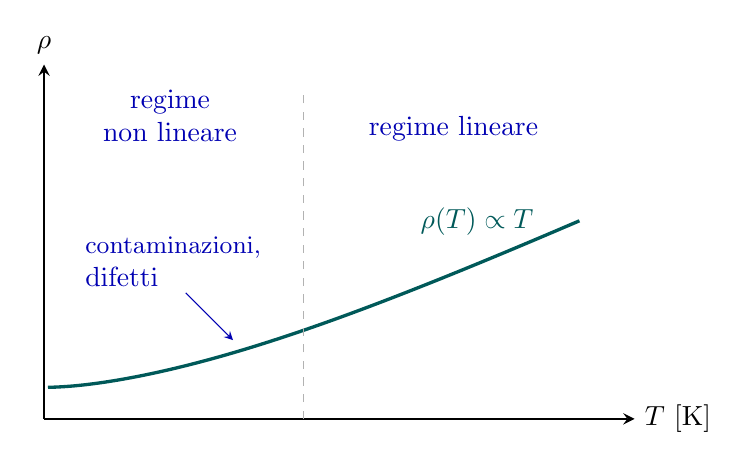
\begin{tikzpicture}[>=stealth, scale=1.0]
        % Assi
        \draw[->, thick] (0, 0) -- (7.5, 0) node[right] {\( T \) [K]};
        \draw[->, thick] (0, 0) -- (0, 4.5) node[above] {\( \rho \)};

        % Curva resistività: piatta a bassa T, poi cresce non linearmente, poi lineare
        \draw[teal!70!black, very thick, smooth, samples=120, domain=0.05:6.8]
            plot (\x, {0.4 + 0.05*\x*\x*exp(-1.2*\x) + 0.45*\x - 0.45*2.2*(1 - exp(-(\x/2.2)))});

        % Separatore fra i due regimi (tratteggio verticale)
        \draw[gray!60, dashed] (3.3, 0) -- (3.3, 4.2);

        % Etichette regimi
        \node[blue!70!black, anchor=south, align=center] at (1.6, 3.4) {regime \\ non lineare};
        \node[blue!70!black, anchor=south] at (5.2, 3.4) {regime lineare};

        % Annotazione \rho \propto T
        \node[teal!70!black] at (5.5, 2.5) {\( \rho(T) \propto T \)};

        % Annotazione cause regime non lineare
        \node[blue!70!black, anchor=west, align=left] at (0.4, 2.0)
            {\small contaminazioni, \\ difetti};
        \draw[->, blue!70!black, thin] (1.8, 1.6) -- (2.4, 1.0);

    \end{tikzpicture}
    \caption{Resistività \( \rho(T) \) di un metallo in funzione della temperatura.}
    \label{fig:resistivita_metallo}
\end{figure}

Nel regime non lineare predominano dunque due classi di imperfezioni:
\begin{itemize}
    \item \textbf{difetti}, ovvero deviazioni dalla struttura cristallina ideale del materiale stesso: assenza di uno o più atomi (vacanze), spostamento degli atomi rispetto alla posizione attesa nel reticolo, dislocazioni (difetti estesi di carattere lineare);
    \item \textbf{contaminazioni}, ossia la presenza di elementi che non appartengono al sistema, atomi estranei sostituzionali o interstiziali introdotti accidentalmente o intenzionalmente nel cristallo.
\end{itemize}
Entrambe queste imperfezioni costituiscono centri di scattering per gli elettroni di conduzione e generano un contributo alla resistività indipendente dalla temperatura, responsabile del valore residuo \( \rho_0 = \rho(T \to 0) \).

La struttura cristallina può dunque presentare deformazioni locali che modificano il potenziale periodico: il potenziale visto dagli elettroni non è più uguale da cella a cella e perde la simmetria di traslazione su cui poggia il teorema di Bloch. A basse temperature è proprio questo meccanismo a dominare la resistività, perché gli atomi del reticolo sono come ``congelati'' nelle loro posizioni e il contributo legato alle vibrazioni reticolari è trascurabile: la conducibilità \( \sigma_e \) è di fatto fissata dai difetti e dalle impurezze presenti nel campione.

Nel regime lineare, ad alte temperature, gli atomi del reticolo iniziano a vibrare e la resistività cresce proporzionalmente a \( T \). Questo regime è dominato dall'interazione degli elettroni di conduzione con le \textbf{vibrazioni reticolari} (fononi), la cui densità aumenta con la temperatura.

\subsubsection{Conducibilità nei metalli reali}

Confrontando l'ordine di grandezza della conducibilità tra metalli e semiconduttori si trova
\begin{equation}
    \sigma_e^{\text{metalli}} \gg \sigma_e^{\text{semicond.}};
\end{equation}
a titolo indicativo, a temperatura ambiente (\( T \sim 20 \divisionsymbol 25 \) \(^{\circ}\)C) i metalli più conduttivi presentano:
\begin{itemize}
    \item rame: \( \sigma_{\text{Cu}} \sim 5{,}9 \times 10^5 \ (\Omega \cdot \text{cm})^{-1} \);
    \item argento: \( \sigma_{\text{Ag}} \sim 6{,}2 \times 10^5 \ (\Omega \cdot \text{cm})^{-1} \);
    \item oro: \( \sigma_{\text{Au}} \sim 4{,}55 \times 10^5 \ (\Omega \cdot \text{cm})^{-1} \).
\end{itemize}
Affinché un materiale mantenga questi valori elevati di conducibilità sono determinanti due aspetti pratici:
\begin{enumerate}
    \item l'assenza di contaminazioni e difetti, che fissa il limite a bassa temperatura della resistività e quindi il valore massimo di \( \sigma_e \) raggiungibile;
    \item la capacità del materiale di preservare nel tempo le proprie proprietà strutturali, resistenza all'ossidazione, alla diffusione di impurezze e all'invecchiamento, in modo che la conducibilità non si degradi durante l'uso.
\end{enumerate}

\begin{remark}
    L'oro è un metallo nobile e non si ossida: non sviluppa cioè uno strato superficiale di ossido, che sarebbe isolante. Argento e rame si ossidano invece entrambi, ma con tempi e intensità diverse: l'argento risulta più sensibile all'ossidazione del rame e per questo motivo, a parità di costo e prestazioni, nei cavi elettrici si preferisce il rame.
\end{remark}

\begin{exercise}
    Si consideri la relazione di dispersione
    \begin{equation}
        E(\vec{k}) = E_0 - 2 \gamma(\vec{R}) \cos(\vec{k} \cdot \vec{R})
    \end{equation}
    dove \( \vec{k} \) è il vettore d'onda e \( \vec{R} = n_1 \vec{a}_1 + n_2 \vec{a}_2 + n_3 \vec{a}_3 \), con \( \vec{a}_1 = a \hat{x} \), \( \vec{a}_2 = a \hat{y} \), \( \vec{a}_3 = a \hat{z} \) (\( \hat{x}, \hat{y}, \hat{z} \) versori cartesiani). Calcolare il tensore della massa efficace \( m_e^* \).
\end{exercise}

\begin{solution}
    Il tensore inverso della massa efficace è dato dall'Hessiana della relazione di dispersione:
    \begin{equation}
        \left( \frac{1}{m_e^*} \right)_{ij} = \frac{1}{\hbar^2} \pdv{E(\vec{k})}{k_i}{k_j} \quad i, j = x, y, z
    \end{equation}
    Per semplicità di notazione poniamo \( \vec{R} = (R_x, R_y, R_z) = (n_1 a, n_2 a, n_3 a) \). Le derivate prime sono
    \begin{align}
        \pdv{E}{k_x} &= 2 \gamma(\vec{R}) \sin(\vec{k} \cdot \vec{R}) \, R_x \\
        \pdv{E}{k_y} &= 2 \gamma(\vec{R}) \sin(\vec{k} \cdot \vec{R}) \, R_y \\
        \pdv{E}{k_z} &= 2 \gamma(\vec{R}) \sin(\vec{k} \cdot \vec{R}) \, R_z
    \end{align}
    ovvero, in forma compatta,
    \begin{equation}
        \pdv{E}{k_i} = 2 \gamma(\vec{R}) \sin(\vec{k} \cdot \vec{R}) \, R_i
    \end{equation}
    Le derivate seconde danno l'Hessiana
    \begin{equation}
        \pdv{E}{k_i}{k_j} = 2 \gamma(\vec{R}) \cos(\vec{k} \cdot \vec{R}) \, R_i R_j
    \end{equation}
    da cui
    \begin{equation}
        \left( \frac{1}{m_e^*} \right)_{ij} = \frac{2 \gamma(\vec{R}) \cos(\vec{k} \cdot \vec{R})}{\hbar^2} \, R_i R_j
    \end{equation}
    Esplicitando la matrice nelle componenti:
    \begin{equation}
        \frac{1}{m_e^*} = \frac{2 \gamma(\vec{R}) \cos(\vec{k} \cdot \vec{R})}{\hbar^2}
        \begin{pmatrix}
            n_1^2 a^2 & n_1 n_2 a^2 & n_1 n_3 a^2 \\
            n_1 n_2 a^2 & n_2^2 a^2 & n_2 n_3 a^2 \\
            n_1 n_3 a^2 & n_2 n_3 a^2 & n_3^2 a^2
        \end{pmatrix}
    \end{equation}

\begin{note}{Invertibilità della matrice}{invmat}
    
    Per ottenere \( m_e^* \) occorre invertire questa matrice, calcolandone la trasposta dei cofattori divisa per il determinante:
    \begin{equation}
        A^{-1} = \frac{C^T}{\det A}
    \end{equation}


\begin{attention}
    Esistono casi in cui la matrice ottenuta è singolare e l'inversa non esiste: localmente la massa efficace diverge lungo certe direzioni cristallografiche, che non sono dunque ammesse come direzioni di moto coerente dell'elettrone.
\end{attention}

Se la matrice \( 1/m_e^* \) può essere ricondotta in forma diagonale tramite una scelta opportuna dei vettori di base, allora, purché il determinante sia non nullo, è invertibile e in quelle direzioni la conducibilità è ben definita. Se invece un'entrata diagonale si annulla, in quella direzione la massa efficace diverge e il materiale non conduce. Considerando ad esempio la forma
\begin{equation}
    \frac{1}{m_e^*} =
    \begin{pmatrix}
        x & 0 & 0 \\
        0 & x & 0 \\
        0 & 0 & 0
    \end{pmatrix}
\end{equation}
il determinante è nullo e l'inversa globale non esiste. Si può tuttavia definire un'\emph{inversa locale}, restringendo l'inversione al sottospazio bidimensionale \( (x, y) \) in cui le entrate diagonali non si annullano: in quella regione la massa efficace è finita e la conduzione è permessa, mentre lungo \( z \) gli elettroni sono effettivamente bloccati. Fisicamente, una struttura di questo tipo descrive materiali a dimensionalità ridotta, ad esempio cristalli stratificati in cui gli elettroni si muovono solo sui piani \( x y \).

\end{note}

    Supponendo il cristallo unidimensionale con \( \vec{R} = n_1 \, \vec{a}_1 \) e \( \vec{a}_1 = a \hat{x} \), è possibile calcolare la massa efficace \( m_e^* \) e la conducibilità \( \sigma_e \).
    Ripercorrendo il calcolo precedente nel caso unidimensionale, la matrice della massa efficace si riduce alla sola componente lungo \( \hat{x} \). Nell'approssimazione tight-binding ai primi vicini si pone \( n_1 = 1 \) (interagisce solo il sito immediatamente adiacente), per cui
    \begin{equation}
        m_e^* = \frac{\hbar^2}{2 \gamma a^2 \cos(k a)}
    \end{equation}
    La conducibilità è data dalla forma di Drude:
    \begin{importantbox}
        \begin{equation}
            \sigma_e = \frac{n_e \, e^2 \, \tau}{m_e^*}
        \end{equation}
    \end{importantbox}
    dove \( n_e \) è la densità di elettroni che effettivamente partecipano alla conduzione. Nei metalli si stima
    \begin{equation}
        n_e = \text{valenza} \cdot n_{\text{at}}
    \end{equation}
    con \( n_{\text{at}} \) densità atomica del materiale. Si tratta di un'approssimazione necessaria a rendere il calcolo praticabile: una valutazione esatta del numero di elettroni di conduzione richiederebbe l'integrazione della distribuzione di Fermi-Dirac sulla banda di conduzione, operazione molto più onerosa.
\end{solution}

\begin{remark}
    Il termine \emph{valenza} ha due significati distinti che non vanno confusi:
    \begin{itemize}
        \item in \textbf{fisica} ``elettroni in banda di valenza'' indica gli elettroni che occupano l'ultima banda piena del cristallo;
        \item in \textbf{chimica} la \emph{valenza} è il numero di elettroni che un atomo mette in compartecipazione per formare un legame chimico.
    \end{itemize}
    Per esempio l'argento ha valenza \( +1 \) (cede un elettrone diventando \( \text{Ag}^+ \)), il rame ha valenza \( +1 \) o \( +2 \) e l'oro valenza \( +1 \). Nella stima \( n_e = \text{valenza} \cdot n_{\text{at}} \) la valenza è intesa in senso chimico: si assume che ciascun atomo contribuisca alla conduzione con un numero di elettroni pari alla sua valenza, ovvero quelli più esterni e meno legati al nucleo. Solo questi elettroni, quelli in banda di conduzione, partecipano effettivamente al trasporto, ed è inutile estendere l'integrale a tutti gli elettroni del cristallo.
\end{remark}

\section{Semiconduttori}

Nei semiconduttori la promozione termica di un elettrone dalla banda di valenza alla banda di conduzione lascia in BV una vacanza, ovvero una \textbf{lacuna}. Vicino al bordo della prima zona di Brillouin, dove si trovano il minimo \( E_c \) della BC e il massimo \( E_v \) della BV, le bande possono essere approssimate in prima istanza da rami di parabola.

\begin{figure}[htbp]
    \centering
    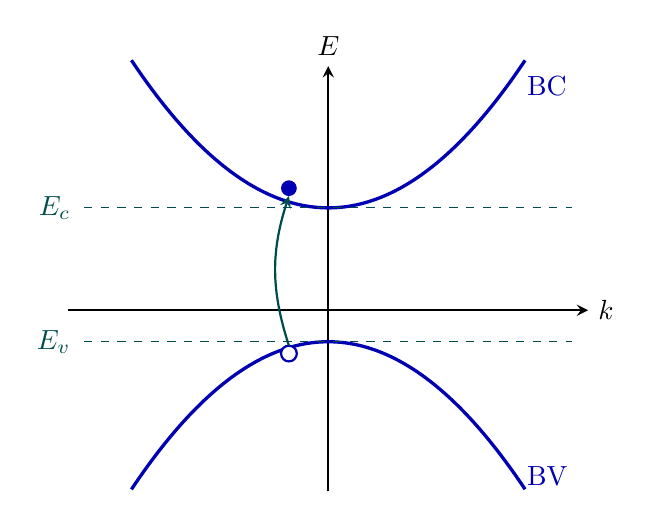
\begin{tikzpicture}[>=stealth, scale=1.0]
        % Assi
        \draw[->, thick] (-3.3, 0) -- (3.3, 0) node[right] {\( k \)};
        \draw[->, thick] (0, -2.3) -- (0, 3.1) node[above] {\( E \)};

        % BC: parabola con minimo in E_c=1.3
        \draw[blue!70!black, very thick, domain=-2.5:2.5, samples=80, smooth]
            plot (\x, {1.3 + 0.3*\x*\x});
        \node[blue!70!black, anchor=west] at (2.4, 2.85) {BC};

        % BV: parabola invertita con massimo in E_v=-0.4
        \draw[blue!70!black, very thick, domain=-2.5:2.5, samples=80, smooth]
            plot (\x, {-0.4 - 0.3*\x*\x});
        \node[blue!70!black, anchor=west] at (2.4, -2.1) {BV};

        % E_c ed E_v
        \draw[teal!60!black, dashed, thin] (-3.1, 1.3) -- (3.1, 1.3);
        \node[teal!60!black, anchor=east] at (-3.15, 1.3) {\( E_c \)};
        \draw[teal!60!black, dashed, thin] (-3.1, -0.4) -- (3.1, -0.4);
        \node[teal!60!black, anchor=east] at (-3.15, -0.4) {\( E_v \)};

        % Elettrone promosso e lacuna
        \fill[blue!70!black] (-0.5, 1.55) circle (0.1);
        \draw[blue!70!black, thick, fill=white] (-0.5, -0.55) circle (0.1);
        \draw[->, teal!60!black, thick] (-0.5, -0.45) to[bend left=18] (-0.5, 1.45);
    \end{tikzpicture}
    \caption{Bande di un semiconduttore in approssimazione parabolica vicino al bordo della zona di Brillouin.}
    \label{fig:bande_paraboliche_semic}
\end{figure}

Il numero \( N_{BC} \) di portatori di carica \( -e \) presenti in BC in un cristallo di volume \( V \) si ottiene contando gli stati occupati dagli elettroni, ovvero pesando la densità degli stati \( g_{BC}(E) \) con la probabilità di occupazione di Fermi-Dirac:
\begin{equation}
    N_{BC} = \int_{E_c}^{\infty} g_{BC}(E) \, f_{FD}(E) \, \dd E
\end{equation}
In prossimità del minimo \( E_c \) la dispersione è quadratica e di conseguenza la densità degli stati ha andamento a radice quadrata,
\begin{equation}
    g_{BC}(E) = B_{BC} \, V \sqrt{E - E_c}
\end{equation}
con \( B_{BC} \) costante che dipende dalla massa efficace dell'elettrone in BC. Sostituendo,
\begin{importantbox}
    \begin{equation}
        N_{BC} = \int_{E_c}^{\infty} B_{BC} \, V \sqrt{E - E_c} \ \frac{1}{\displaystyle e^{(E - \mu)/k_B T} + 1} \, \dd E
    \end{equation}
\end{importantbox}

Il potenziale chimico \( \mu \) che compare nella Fermi-Dirac è il livello energetico al quale la probabilità di occupazione vale \( 1/2 \), cioè \( f_{FD}(\mu) = 1/2 \). Nei metalli a \( T = 0 \) K esso coincide con l'energia del massimo livello occupato, \( \mu(T = 0) = E_F \), e si parla di \textbf{energia di Fermi}. Nel semiconduttore \( \mu \) cade invece all'interno del gap, in una regione priva di stati: la definizione di Fermi come ``livello dell'ultimo stato occupato'' perde di significato e \( \mu \) resta solo un parametro statistico.

\begin{figure}[htbp]
    \centering
    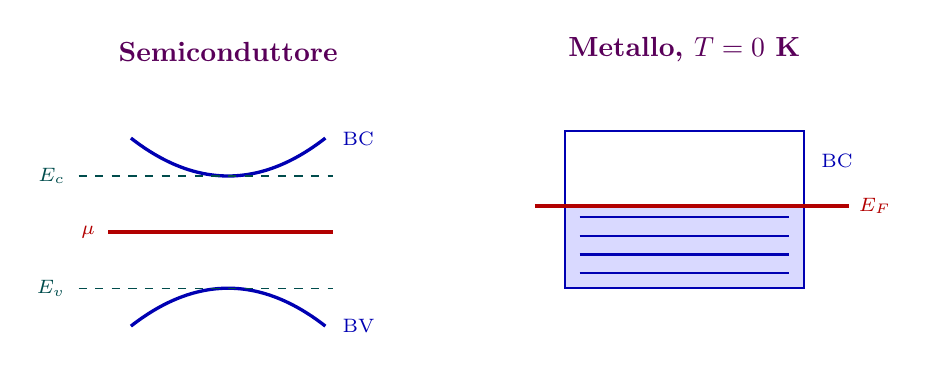
\begin{tikzpicture}[>=stealth, scale=0.95]
        % ===== SEMICONDUTTORE =====
        \def\xMs{-2.5}

        \node[violet!70!black, font=\bfseries, anchor=south] at (\xMs, 2.6) {Semiconduttore};

        % BC e BV (parabole)
        \draw[blue!70!black, very thick, domain=-1.3:1.3, samples=60, smooth]
            plot ({\xMs+\x}, {1.2 + 0.3*\x*\x});
        \draw[blue!70!black, very thick, domain=-1.3:1.3, samples=60, smooth]
            plot ({\xMs+\x}, {-0.3 - 0.3*\x*\x});
        \node[blue!70!black, anchor=west, font=\scriptsize] at (\xMs+1.4, 1.7) {BC};
        \node[blue!70!black, anchor=west, font=\scriptsize] at (\xMs+1.4, -0.8) {BV};

        % E_c, E_v
        \draw[teal!60!black, dashed, thin] (\xMs-2.0, 1.2) -- (\xMs+1.4, 1.2);
        \node[teal!60!black, anchor=east, font=\scriptsize] at (\xMs-2.05, 1.2) {\( E_c \)};
        \draw[teal!60!black, dashed, thin] (\xMs-2.0, -0.3) -- (\xMs+1.4, -0.3);
        \node[teal!60!black, anchor=east, font=\scriptsize] at (\xMs-2.05, -0.3) {\( E_v \)};

        % mu nel gap
        \draw[red!70!black, very thick] (\xMs-1.6, 0.45) -- (\xMs+1.4, 0.45);
        \node[red!70!black, anchor=east, font=\scriptsize] at (\xMs-1.65, 0.45) {\( \mu \)};

        % ===== METALLO =====
        \def\xLm{2.0}
        \def\xRm{5.2}

        \node[violet!70!black, font=\bfseries, anchor=south] at ({(\xLm+\xRm)/2}, 2.6) {Metallo, \( T = 0 \) K};

        \fill[blue!15] (\xLm, -0.3) rectangle (\xRm, 0.8);
        \draw[blue!70!black, thick] (\xLm, -0.3) rectangle (\xRm, 1.8);
        \foreach \y in {-0.1, 0.15, 0.4, 0.65} {
            \draw[blue!70!black, thick] (\xLm+0.2, \y) -- (\xRm-0.2, \y);
        }
        \node[blue!70!black, anchor=west, font=\scriptsize] at (\xRm+0.1, 1.4) {BC};

        \draw[red!70!black, very thick] (\xLm-0.4, 0.8) -- (\xRm+0.6, 0.8);
        \node[red!70!black, anchor=west, font=\scriptsize] at (\xRm+0.6, 0.8) {\( E_F \)};
    \end{tikzpicture}
    \caption{Posizione di \( \mu \) in un semiconduttore e di \( E_F \) in un metallo a \( T = 0 \) K.}
    \label{fig:mu_semicond_metallo}
\end{figure}

Nel semiconduttore vale la condizione
\begin{equation}
    E - \mu \gg k_B T \qquad \text{per ogni } E \ge E_c
\end{equation}
dove \( k_B T \) è l'energia termica caratteristica. Fisicamente significa che l'energia termica disponibile è troppo bassa per compiere il salto energetico necessario a popolare i livelli sopra il gap. Di conseguenza l'esponenziale al denominatore della Fermi-Dirac domina sull'unità,
\begin{equation}
    e^{(E - \mu)/k_B T} + 1 \ \simeq \ e^{(E - \mu)/k_B T}
\end{equation}
e la distribuzione si riduce a una Boltzmann. L'integrale per \( N_{BC} \) diventa
\begin{equation}
    N_{BC} = \int_{E_c}^{\infty} B_{BC} \, V \sqrt{E - E_c} \ e^{-(E - \mu)/k_B T} \, \dd E
\end{equation}
che si risolve con il cambio di variabile \(x = \frac{E - \mu}{k_B T}\).

Risolvendo si ottiene la densità di elettroni in BC:
\begin{importantbox}
    \begin{equation}
        n_{BC} = \frac{N_{BC}}{V} = K_{BC}(T) \, e^{-(E_c - \mu)/k_B T}
        \qquad
        K_{BC}(T) = \frac{1}{4} \left( \frac{2 m_e^* k_B T}{\pi \hbar^2} \right)^{3/2}
    \end{equation}
\end{importantbox}

In modo del tutto analogo si calcola il numero di \textbf{lacune} (vacanze) in banda di valenza, pesando la densità degli stati con la probabilità che lo stato sia \emph{non} occupato, ovvero \( 1 - f_{FD}(E) \):
\begin{equation}
    P_{BV} = \int_{-\infty}^{E_v} g_{BV}(E) \, \bigl( 1 - f_{FD}(E) \bigr) \, \dd E
\end{equation}
Sviluppando la dispersione attorno al massimo della BV in approssimazione parabolica, la densità degli stati assume la forma
\begin{equation}
    g_{BV}(E) = B_{BV} \, V \sqrt{E_v - E}
\end{equation}
con \( B_{BV} \) costante che dipende dalla massa efficace della lacuna \( m_v^* \) (in generale diversa dalla massa efficace dell'elettrone in BC, \( m_v^* \ne m_e^* \)).

Per creare una lacuna serve portare via un elettrone dalla BV: più ci si addentra in profondità nella banda, verso valori di \( E \) sempre più piccoli, più \( \mu - E \) diventa grande e più costoso è il processo. Poiché l'energia termica \( k_B T \) è molto minore di \( \mu - E \), il numero di lacune presenti diminuisce esponenzialmente man mano che ci si allontana dal bordo \( E_v \) verso il fondo della banda: le lacune restano quindi concentrate quasi tutte vicino al massimo della BV.

In modo speculare al caso della BC vale la condizione
\begin{equation}
    \mu - E \gg k_B T \qquad \text{per ogni } E \le E_v
\end{equation}
che permette di approssimare il denominatore della Fermi-Dirac come
\begin{equation}
    e^{(E - \mu)/k_B T} + 1 = e^{-(\mu - E)/k_B T} + 1 \ \simeq \ 1
\end{equation}
Riscrivendo \( 1 - f_{FD} \) nella forma
\begin{equation}
    1 - f_{FD}(E) = \frac{e^{(E - \mu)/k_B T} + 1 - 1}{e^{(E - \mu)/k_B T} + 1}
\end{equation}
il numero di lacune assume infine la forma
\begin{equation}
    P_{BV} = \int_{-\infty}^{E_v} B_{BV} \, V \sqrt{E_v - E} \, \frac{e^{(E - \mu)/k_B T} + 1 - 1}{e^{(E - \mu)/k_B T} + 1} \, \dd E
\end{equation}

Risolvendo si ottiene la densità di lacune in BV:
\begin{importantbox}
    \begin{equation}
        p_{BV} = \frac{P_{BV}}{V} = K_{BV}(T) \, e^{-(\mu - E_v)/k_B T}
        \qquad
        K_{BV}(T) = \frac{1}{4} \left( \frac{2 m_v^* k_B T}{\pi \hbar^2} \right)^{3/2}
    \end{equation}
\end{importantbox}
con la massa efficace della lacuna definita, in modo analogo a quella dell'elettrone, dall'Hessiana della relazione di dispersione attorno al massimo della BV:
\begin{equation}
    \left( \frac{1}{m_v^*} \right)_{ij} = \frac{1}{\hbar^2} \pdv{E_{BV}}{k_i}{k_j} \qquad \frac{1}{m_v^*} \ne \frac{1}{m_e^*}
\end{equation}

In un \textbf{semiconduttore intrinseco} (privo di drogaggio) ogni elettrone promosso in BC lascia esattamente una lacuna in BV: il numero di elettroni in BC è pari al numero di lacune in BV, e si introduce la \textbf{concentrazione intrinseca}
\begin{equation}
    n_{BC} = p_{BV} \eqqcolon n_i
\end{equation}
Esplicitando le due espressioni si ottiene la condizione
\begin{importantbox}
    \begin{equation}
        K_{BC}(T) \, e^{-(E_c - \mu)/k_B T} = K_{BV}(T) \, e^{-(\mu - E_v)/k_B T}
    \end{equation}
\end{importantbox}

Riordinando i fattori esponenziali si trova
\begin{align}
    \frac{K_{BC}(T)}{K_{BV}(T)} &= e^{(E_v - \mu)/k_B T} \, e^{(E_c - \mu)/k_B T} = e^{(E_v + E_c - 2\mu)/k_B T}
\end{align}
Dalla forma esplicita dei prefattori si ricava inoltre
\begin{equation}
    \frac{K_{BC}(T)}{K_{BV}(T)} = \left( \frac{m_e^*}{m_v^*} \right)^{3/2}
\end{equation}
Uguagliando le due espressioni e prendendo il logaritmo si ottiene infine il potenziale chimico del semiconduttore intrinseco:
\begin{importantbox}
    \begin{equation}
        \mu(T) = \frac{3}{4} k_B T \ln\!\left( \frac{m_v^*}{m_e^*} \right) + \frac{E_g}{2} + E_v
    \end{equation}
\end{importantbox}
A \( T = 0 \), o quando le due masse efficaci coincidono, \( \mu \) si trova esattamente al centro del gap, \( \mu = E_v + E_g/2 \); la dipendenza da \( T \) e dal rapporto fra le masse efficaci sposta leggermente \( \mu \) dal punto medio.

\begin{remark}
    Il potenziale chimico \( \mu \), per definizione, ha le dimensioni di un'energia.
\end{remark}

Moltiplicando le due concentrazioni \( n_{BC} \) e \( p_{BV} \) le dipendenze da \( \mu \) si elidono:
\begin{align}
    n_i^2 = n_{BC} \cdot p_{BV}
        &= K_{BC}(T) \, e^{-(E_c - \mu)/k_B T} \cdot K_{BV}(T) \, e^{-(\mu - E_v)/k_B T} \notag \\
        &= K_{BC}(T) \, K_{BV}(T) \, e^{-(E_c - E_v)/k_B T}
\end{align}
ovvero, ricordando che \( E_c - E_v = E_g \), la \textbf{legge di azione di massa}:
\begin{importantbox}
    \begin{equation}
        n_i^2 = K_{BC}(T) \, K_{BV}(T) \, e^{-E_g/k_B T}
    \end{equation}
    \begin{equation}
        n_i = \sqrt{K_{BC}(T) \, K_{BV}(T)} \ e^{-E_g/(2 k_B T)}
    \end{equation}
\end{importantbox}
La concentrazione intrinseca dipende dunque esclusivamente dal gap del materiale e dalla temperatura, e non dalla posizione di \( \mu \).

Nei semiconduttori sono dunque presenti due tipi di portatori di carica, elettroni e lacune, che contribuiscono entrambi al trasporto. Nei semiconduttori intrinseci (ad esempio Si, Ge) partecipano alla conducibilità sia gli elettroni in BC sia le lacune in BV. Applicando un campo elettrico \( \vec{E} \), la densità di corrente totale è la somma dei due contributi:
\begin{align}
    \vec{J} &= \vec{J}_{e, BC} + \vec{J}_{v, BV} \notag \\
        &= \sigma_{e, BC} \vec{E} + \sigma_{v, BV} \vec{E} = \sigma_{\text{semic}} \vec{E}
\end{align}
con
\begin{equation}
    \sigma_{\text{semic}} \coloneqq \sigma_{e, BC} + \sigma_{v, BV}
\end{equation}
e
\begin{equation}
    \sigma_{e, BC} = \frac{n_{e, BC} \, e^2 \, \tau_{BC}}{m_e^*}
    \qquad
    \sigma_{v, BV} = \frac{p_{v, BV} \, e^2 \, \tau_{BV}}{m_v^*}
\end{equation}

Similmente al caso dei metalli si definiscono le mobilità dei due portatori:
\begin{equation}
    \mu_{e, BC} = -\frac{e \, \tau_{BC}}{m_e^*}
    \qquad
    \mu_{v, BV} = +\frac{e \, \tau_{BV}}{m_v^*}
\end{equation}
con segni opposti che riflettono la carica opposta di elettroni e lacune.

Nel caso del semiconduttore intrinseco la resistività si ottiene invertendo la conducibilità totale:
\begin{equation}
    \rho = \frac{1}{\sigma_{\text{semic}}} = \frac{1}{\dfrac{n_{e, BC} \, e^2 \, \tau_{BC}}{m_e^*} + \dfrac{p_{v, BV} \, e^2 \, \tau_{BV}}{m_v^*}}
\end{equation}
Sfruttando la condizione \( n_{e, BC} = p_{v, BV} = n_i \) tipica del semiconduttore intrinseco, l'espressione si semplifica in
\begin{importantbox}
    \begin{equation}
        \rho = \frac{1}{n_i \, e^2 \left( \dfrac{\tau_{BC}}{m_e^*} + \dfrac{\tau_{BV}}{m_v^*} \right)}
    \end{equation}
\end{importantbox}

\begin{attention}
    Nel semiconduttore intrinseco \( n_i = n_{e, BC} = p_{v, BV} \), a temperatura fissata, è una costante che dipende solo dal gap e dalle masse efficaci dei portatori.
\end{attention}

\subsection{Corrente di diffusione}

\lezione{22}{18/05/2026}

Finora abbiamo considerato un campione omogeneo, in cui la concentrazione dei portatori è uniforme. Se invece due materiali con concentrazioni differenti vengono messi a contatto, all'interfaccia si stabilisce una distribuzione non uniforme dei portatori che tende a riequilibrarsi nel tempo: in presenza di un gradiente di concentrazione i portatori si spostano spontaneamente dalle regioni più popolate a quelle meno popolate, generando una densità di corrente detta \textbf{corrente di diffusione}.

Per gli elettroni (portatori di carica negativa) la densità di corrente di diffusione è proporzionale al gradiente della concentrazione \( n \):
\begin{importantbox}
    \begin{equation}
        \vec{J}_e = \vec{J}_n = -e \, D_n \, \vec{\nabla} n
    \end{equation}
\end{importantbox}
dove:
\begin{itemize}
    \item \( n \) è la densità di portatori di carica negativa (elettroni in BC);
    \item \( D_n \) è il \textbf{coefficiente di diffusione} degli elettroni, che misura la capacità dei portatori di ridurre il gradiente di concentrazione;
    \item il segno meno tiene conto della carica negativa dell'elettrone e del fatto che la corrente di diffusione si oppone al gradiente.
\end{itemize}
Lungo un singolo asse, ad esempio \( \hat{x} \), la relazione si riduce alla componente
\begin{equation}
    J_{n, x} = -e \, D_n \, \pdv{n}{x}
\end{equation}

In modo del tutto analogo si scrive la corrente di diffusione delle \textbf{lacune}, portatori di carica positiva:
\begin{importantbox}
    \begin{equation}
        \vec{J}_p = \vec{J}_v = e \, D_p \, \vec{\nabla} p
    \end{equation}
\end{importantbox}
dove \( p \) è la densità delle lacune in BV e \( D_p \) il loro coefficiente di diffusione. Il segno positivo riflette la carica opposta del portatore rispetto all'elettrone.

Quando un materiale non è omogeneo, vuoi per ragioni intrinseche, vuoi per modifiche introdotte in laboratorio, occorre tenere conto del fatto che la variazione locale della struttura altera le proprietà elettriche del campione, e in particolare la capacità dei portatori di diffondere.

Mobilità e coefficiente di diffusione non sono grandezze indipendenti: entrambi misurano la facilità con cui un portatore di carica si muove sotto due forze diverse, il campo elettrico nel caso della mobilità e il gradiente di concentrazione nel caso del coefficiente di diffusione. Einstein dimostrò che le due grandezze sono legate dalla \textbf{relazione di Einstein}, che per un portatore di carica \( q \), mobilità \( \mu_q \) e coefficiente di diffusione \( D_q \) si scrive
\begin{importantbox}
    \begin{equation}
        \frac{D_q}{\mu_q} = \frac{k_B T}{q}
    \end{equation}
\end{importantbox}
con \( T \) la temperatura del campione.

L'interpretazione fisica della relazione è duplice:
\begin{itemize}
    \item al crescere della temperatura aumenta l'energia termica \( k_B T \) disponibile per i portatori e di conseguenza aumenta la loro capacità di diffondere all'interno del materiale;
    \item al crescere della densità di carica locale aumenta il campo elettrico interno che essa stessa genera, il quale deforma la simmetria del reticolo nelle immediate vicinanze. Questa deformazione si traduce in un \emph{attrito efficace} maggiore per i portatori, che devono spendere più energia per spostarsi: la diffusione risulta dunque inibita dall'eccesso locale di carica.
\end{itemize}

Nel semiconduttore intrinseco la conducibilità cresce con la concentrazione \( n_i \) dei portatori: la legge di azione di massa fissa il valore di \( n_i \) e con esso il livello di conducibilità raggiungibile.

\begin{figure}[htbp]
    \centering
    \begin{tikzpicture}[>=stealth, scale=1.0]
        \draw[->, thick] (0, 0) -- (7.5, 0) node[right, align=center, font=\scriptsize] {concentrazione \\ port. di carica \( n_i \) \\ \( [\text{cm}^{-3}] \)};
        \draw[->, thick] (0, 0) -- (0, 4.2) node[above] {\( \sigma \)};

        \draw[blue!70!black, very thick, smooth, samples=120, domain=0.4:5.8]
            plot (\x, {0.15*exp(0.55*\x)});

        \draw[gray!60, dashed] (1.2, 0) -- (1.2, 0.3);
        \draw[gray!60, dashed] (3.6, 0) -- (3.6, 1.1);
        \node[anchor=north, font=\scriptsize] at (1.2, -0.05) {\( 10^{10} \)};
        \node[anchor=north, font=\scriptsize] at (3.6, -0.05) {\( 10^{14} \)};
    \end{tikzpicture}
    \caption{Conducibilità di un semiconduttore intrinseco in funzione della concentrazione di portatori \( n_i \).}
    \label{fig:sigma_ni_intrinseco}
\end{figure}

\begin{exercise}
    Verificare l'ordine di grandezza della densità di elettroni in BC per un semiconduttore intrinseco di silicio a temperatura ambiente \( T = 25 \) \(^\circ\)C, sapendo che il gap del Si vale \( E_{g,\text{Si}} \simeq 1{,}12 \) eV.
\end{exercise}

\subsection{Semiconduttori drogati}

Il \textbf{drogaggio} (doping) di un semiconduttore consiste nella modifica controllata della sua composizione, incorporando nel cristallo ospite un elemento diverso da quello di base. Le concentrazioni tipiche di drogante si collocano nell'intervallo
\begin{equation}
    10^{14} \divisionsymbol 10^{18} \ \text{atomi/cm}^3
\end{equation}
da confrontare con la densità atomica caratteristica di una mole di materiale, \( \sim 10^{23} \) atomi/cm\(^3\): l'elemento estraneo costituisce quindi una piccola frazione del totale.

In base alla concentrazione introdotta si distinguono due regimi:
\begin{itemize}
    \item \textbf{contaminante} se la concentrazione è inferiore a \( 10^{13} \) atomi/cm\(^3\);
    \item \textbf{drogante} se la concentrazione è superiore o uguale a \( 10^{14} \) atomi/cm\(^3\).
\end{itemize}
La distinzione non è solo terminologica: nel regime contaminante l'elemento estraneo agisce come centro di scattering occasionale e modifica poco le proprietà elettriche del materiale, mentre nel regime di drogaggio vero e proprio le sue impurezze determinano in modo dominante la densità di portatori liberi.

In un semiconduttore drogato la densità di portatori di carica dipende dalla temperatura in modo caratteristico: tracciando \( n \) in funzione di \( 1/T \) si distinguono tre regimi successivi.

\begin{figure}[H]
    \centering
    \begin{tikzpicture}[>=stealth, scale=1.0]
        \draw[->, thick] (0, 0) -- (11, 0) node[right] {\( 1000/T \) [1/K]};
        \draw[->, thick] (0, 0) -- (0, 5.8) node[above, align=center, font=\scriptsize] {dens. port. \\ carica};

        \def\hpa{3.1}
        \def\hpb{2.3}

        \draw[teal!70!black, very thick, smooth, samples=160, domain=0.45:2.5]
            plot (\x, {\hpa + 0.7*(2.5-\x)*(2.5-\x)});
        \draw[teal!70!black, very thick] (2.5, \hpa) -- (8.5, \hpb);
        \draw[teal!70!black, very thick, smooth, samples=160, domain=8.5:10.4]
            plot (\x, {\hpb*exp(-1.4*(\x-8.5)*(\x-8.5))});

        \draw[gray!60, dashed] (2.5, 0) -- (2.5, 5.4);
        \draw[gray!60, dashed] (8.5, 0) -- (8.5, \hpb + 0.4);
        \node[anchor=north, font=\scriptsize] at (2.5, -0.05) {\( 2 \)};
        \node[anchor=north, font=\scriptsize] at (8.5, -0.05) {\( 8 \)};

        \node[blue!70!black, font=\scriptsize, anchor=south, align=center] at (1.4, 1.6) {regime \\ intrinseco};
        \node[blue!70!black, font=\scriptsize, anchor=south, align=center] at (5.5, 1.6) {regime di \\ saturazione};
        \node[blue!70!black, font=\scriptsize, anchor=south, align=center] at (9.8, 1.8) {freeze-out};
    \end{tikzpicture}
    \caption{Densità di portatori di carica in un semiconduttore drogato in funzione di \( 1000/T \).}
    \label{fig:regimi_drogato}
\end{figure}

I tre regimi corrispondono a tre meccanismi distinti di popolamento della banda di conduzione:
\begin{itemize}
    \item \textbf{regime intrinseco} (alta temperatura, \( k_B T \sim E_g \)): l'energia termica è sufficiente a promuovere un gran numero di elettroni della banda di valenza del materiale ospite alla banda di conduzione, vengono ``spezzati'' atomi di silicio in numero molto maggiore di quelli del drogante. La densità intrinseca soddisfa \( n_i \gg N_D \), dove \( N_D \) è la densità di drogante, e il contributo delle impurezze diventa irrilevante: il sistema si comporta come un semiconduttore intrinseco;
    \item \textbf{regime di saturazione} (temperatura intermedia): la temperatura è abbastanza alta da ionizzare completamente gli atomi droganti, ma resta troppo bassa per spezzare in modo significativo i legami del materiale ospite. La densità di portatori coincide allora con la densità di drogante e rimane circa costante al variare di \( T \);
    \item \textbf{regime di freeze-out} (bassa temperatura, \( k_B T < E_{\text{ioniz}} \)): l'energia termica non basta a ionizzare gli atomi droganti e gli elettroni restano localizzati attorno agli atomi donori. La densità di portatori liberi crolla esponenzialmente al diminuire di \( T \).
\end{itemize}

In base alla valenza del drogante rispetto a quella del materiale ospite si distinguono due tipi fondamentali di drogaggio. In entrambi i casi il sistema resta complessivamente neutro: il drogante non aggiunge carica netta, ma rende disponibili portatori liberi spostando il bilancio fra elettroni in banda di conduzione e lacune in banda di valenza.

\subsubsection{Drogaggio di tipo \texorpdfstring{\( n \)}{n} (donori)}

Si considera un semiconduttore intrinseco drogato con un elemento di \emph{valenza maggiore} di quella dell'ospite. Il caso prototipo è il silicio (Si\(^{4+}\)) drogato con arsenico (As\(^{5+}\)): il silicio impegna quattro elettroni nei legami covalenti con i quattro vicini più prossimi, mentre l'arsenico ne porta cinque. I primi quattro elettroni dell'As partecipano ai legami con i quattro atomi di Si circostanti, mentre il quinto rimane debolmente legato all'atomo di As e funge da \textbf{elettrone donore}, facilmente promosso in banda di conduzione.

A livello di struttura a bande il drogaggio introduce un nuovo livello energetico \( E_D \) localizzato appena al di sotto del bordo \( E_c \) della banda di conduzione: a \( T = 0 \) K il livello donore è occupato, a \( T \neq 0 \) K l'energia termica è sufficiente a promuovere l'elettrone donore in BC.

\begin{figure}[htbp]
    \centering
    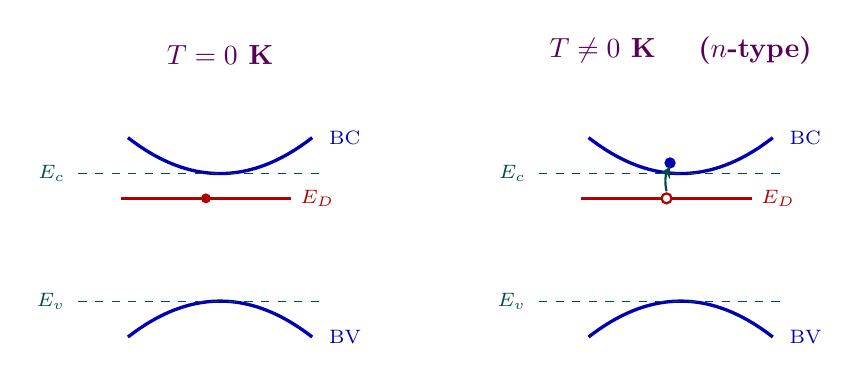
\begin{tikzpicture}[>=stealth, scale=0.9]
        % ===== T = 0 K =====
        \def\xL{-3.0}
        \node[violet!70!black, font=\bfseries, anchor=south] at (\xL, 2.8) {\( T = 0 \) K};

        \draw[blue!70!black, very thick, domain=-1.3:1.3, samples=60, smooth]
            plot ({\xL+\x}, {1.4 + 0.3*\x*\x});
        \draw[blue!70!black, very thick, domain=-1.3:1.3, samples=60, smooth]
            plot ({\xL+\x}, {-0.4 - 0.3*\x*\x});
        \node[blue!70!black, anchor=west, font=\scriptsize] at (\xL+1.4, 1.9) {BC};
        \node[blue!70!black, anchor=west, font=\scriptsize] at (\xL+1.4, -0.9) {BV};

        \draw[teal!60!black, dashed, thin] (\xL-2.0, 1.4) -- (\xL+1.4, 1.4);
        \node[teal!60!black, anchor=east, font=\scriptsize] at (\xL-2.05, 1.4) {\( E_c \)};
        \draw[teal!60!black, dashed, thin] (\xL-2.0, -0.4) -- (\xL+1.4, -0.4);
        \node[teal!60!black, anchor=east, font=\scriptsize] at (\xL-2.05, -0.4) {\( E_v \)};

        \draw[red!70!black, very thick] (\xL-1.4, 1.05) -- (\xL+1.0, 1.05);
        \node[red!70!black, anchor=west, font=\scriptsize] at (\xL+1.0, 1.05) {\( E_D \)};
        \fill[red!70!black] (\xL-0.2, 1.05) circle (0.07);

        % ===== T != 0 K =====
        \def\xR{3.5}
        \node[violet!70!black, font=\bfseries, anchor=south] at (\xR, 2.8) {\( T \neq 0 \) K \quad ($n$-type)};

        \draw[blue!70!black, very thick, domain=-1.3:1.3, samples=60, smooth]
            plot ({\xR+\x}, {1.4 + 0.3*\x*\x});
        \draw[blue!70!black, very thick, domain=-1.3:1.3, samples=60, smooth]
            plot ({\xR+\x}, {-0.4 - 0.3*\x*\x});
        \node[blue!70!black, anchor=west, font=\scriptsize] at (\xR+1.4, 1.9) {BC};
        \node[blue!70!black, anchor=west, font=\scriptsize] at (\xR+1.4, -0.9) {BV};

        \draw[teal!60!black, dashed, thin] (\xR-2.0, 1.4) -- (\xR+1.4, 1.4);
        \node[teal!60!black, anchor=east, font=\scriptsize] at (\xR-2.05, 1.4) {\( E_c \)};
        \draw[teal!60!black, dashed, thin] (\xR-2.0, -0.4) -- (\xR+1.4, -0.4);
        \node[teal!60!black, anchor=east, font=\scriptsize] at (\xR-2.05, -0.4) {\( E_v \)};

        \draw[red!70!black, very thick] (\xR-1.4, 1.05) -- (\xR+1.0, 1.05);
        \node[red!70!black, anchor=west, font=\scriptsize] at (\xR+1.0, 1.05) {\( E_D \)};

        % electron promoted to BC
        \fill[blue!70!black] (\xR-0.15, 1.55) circle (0.08);
        \draw[->, teal!60!black, thick] (\xR-0.2, 1.15) to[bend left=20] (\xR-0.15, 1.5);
        \draw[red!70!black, thick, fill=white] (\xR-0.2, 1.05) circle (0.07);
    \end{tikzpicture}
    \caption{Struttura a bande di un semiconduttore con drogaggio di tipo \( n \) (donore): il livello donore \( E_D \) si colloca appena sotto \( E_c \) e a \( T \neq 0 \) K l'elettrone donore viene promosso in banda di conduzione.}
    \label{fig:drogaggio_n_type}
\end{figure}

Il bilancio dei portatori in banda di conduzione include allora sia gli elettroni promossi termicamente dal materiale ospite (concentrazione intrinseca \( n_i \)) sia quelli ceduti dagli atomi donori ionizzati, di concentrazione \( N_D^+ \):
\begin{equation}
    n_{e, BC} = n_i + N_D^+
\end{equation}
dove \( N_D^+ \) rappresenta il numero di donori che hanno effettivamente ceduto il proprio elettrone in BC.

Nelle condizioni tipiche di drogaggio, \( N_D \sim 10^{15} \divisionsymbol 10^{18} \) atomi/cm\(^3\), nel regime di saturazione il contributo dei donori domina su quello intrinseco e si ha
\begin{importantbox}
    \begin{equation}
        n_{e, BC} \simeq N_D^+
    \end{equation}
\end{importantbox}
Il materiale così ottenuto si dice drogato \textbf{\( n \)-type}: i portatori di carica dominanti sono elettroni in banda di conduzione.

\subsubsection{Drogaggio di tipo \texorpdfstring{\( p \)}{p} (accettori)}

Speculare al caso precedente è il drogaggio con un elemento di \emph{valenza inferiore} a quella dell'ospite. Per il silicio (Si\(^{4+}\)) un esempio tipico è il boro (B\(^{3+}\)): il boro porta soltanto tre elettroni di valenza, uno in meno rispetto ai quattro che il silicio impegna nei legami covalenti. Il legame con uno dei quattro vicini di Si resta dunque incompleto e l'atomo di boro funge da \textbf{accettore}: può catturare un elettrone dalla banda di valenza, lasciando in essa una lacuna libera di propagarsi. Anche in questo caso il sistema resta complessivamente neutro dopo il drogaggio.

A livello di struttura a bande il drogaggio di tipo \( p \) introduce un livello accettore \( E_A \) localizzato appena al di sopra del bordo \( E_v \) della banda di valenza: a \( T \neq 0 \) K un elettrone della BV viene catturato dall'accettore, lasciando una lacuna in BV.

\begin{figure}[htbp]
    \centering
    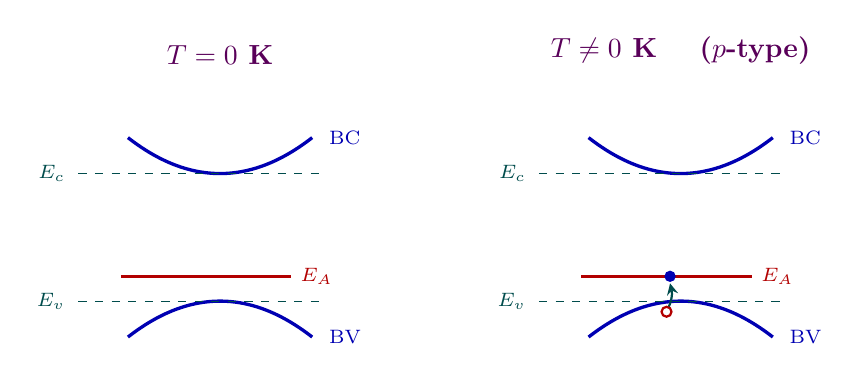
\begin{tikzpicture}[>=stealth, scale=0.9]
        % ===== T = 0 K =====
        \def\xL{-3.0}
        \node[violet!70!black, font=\bfseries, anchor=south] at (\xL, 2.8) {\( T = 0 \) K};

        \draw[blue!70!black, very thick, domain=-1.3:1.3, samples=60, smooth]
            plot ({\xL+\x}, {1.4 + 0.3*\x*\x});
        \draw[blue!70!black, very thick, domain=-1.3:1.3, samples=60, smooth]
            plot ({\xL+\x}, {-0.4 - 0.3*\x*\x});
        \node[blue!70!black, anchor=west, font=\scriptsize] at (\xL+1.4, 1.9) {BC};
        \node[blue!70!black, anchor=west, font=\scriptsize] at (\xL+1.4, -0.9) {BV};

        \draw[teal!60!black, dashed, thin] (\xL-2.0, 1.4) -- (\xL+1.4, 1.4);
        \node[teal!60!black, anchor=east, font=\scriptsize] at (\xL-2.05, 1.4) {\( E_c \)};
        \draw[teal!60!black, dashed, thin] (\xL-2.0, -0.4) -- (\xL+1.4, -0.4);
        \node[teal!60!black, anchor=east, font=\scriptsize] at (\xL-2.05, -0.4) {\( E_v \)};

        \draw[red!70!black, very thick] (\xL-1.4, -0.05) -- (\xL+1.0, -0.05);
        \node[red!70!black, anchor=west, font=\scriptsize] at (\xL+1.0, -0.05) {\( E_A \)};

        % ===== T != 0 K =====
        \def\xR{3.5}
        \node[violet!70!black, font=\bfseries, anchor=south] at (\xR, 2.8) {\( T \neq 0 \) K \quad ($p$-type)};

        \draw[blue!70!black, very thick, domain=-1.3:1.3, samples=60, smooth]
            plot ({\xR+\x}, {1.4 + 0.3*\x*\x});
        \draw[blue!70!black, very thick, domain=-1.3:1.3, samples=60, smooth]
            plot ({\xR+\x}, {-0.4 - 0.3*\x*\x});
        \node[blue!70!black, anchor=west, font=\scriptsize] at (\xR+1.4, 1.9) {BC};
        \node[blue!70!black, anchor=west, font=\scriptsize] at (\xR+1.4, -0.9) {BV};

        \draw[teal!60!black, dashed, thin] (\xR-2.0, 1.4) -- (\xR+1.4, 1.4);
        \node[teal!60!black, anchor=east, font=\scriptsize] at (\xR-2.05, 1.4) {\( E_c \)};
        \draw[teal!60!black, dashed, thin] (\xR-2.0, -0.4) -- (\xR+1.4, -0.4);
        \node[teal!60!black, anchor=east, font=\scriptsize] at (\xR-2.05, -0.4) {\( E_v \)};

        \draw[red!70!black, very thick] (\xR-1.4, -0.05) -- (\xR+1.0, -0.05);
        \node[red!70!black, anchor=west, font=\scriptsize] at (\xR+1.0, -0.05) {\( E_A \)};

        % electron captured to acceptor level, hole left in BV
        \fill[blue!70!black] (\xR-0.15, -0.05) circle (0.08);
        \draw[->, teal!60!black, thick] (\xR-0.2, -0.55) to[bend right=20] (\xR-0.15, -0.15);
        \draw[red!70!black, thick, fill=white] (\xR-0.2, -0.55) circle (0.07);
    \end{tikzpicture}
    \caption{Struttura a bande di un semiconduttore con drogaggio di tipo \( p \) (accettore): il livello accettore \( E_A \) si colloca appena sopra \( E_v \) e a \( T \neq 0 \) K cattura un elettrone dalla BV lasciandovi una lacuna.}
    \label{fig:drogaggio_p_type}
\end{figure}

Il numero di stati ionizzati di tipo accettore (che hanno ricevuto un elettrone) si indica con \( N_A^- \). Il bilancio delle lacune in banda di valenza diventa
\begin{equation}
    p_{v, BV} = n_i + N_A^-
\end{equation}
e nel regime di saturazione, in cui \( N_A^- \gg n_i \), si ha
\begin{importantbox}
    \begin{equation}
        p_{v, BV} \simeq N_A^-
    \end{equation}
\end{importantbox}
Il materiale si dice drogato \textbf{\( p \)-type}: i portatori di carica dominanti sono lacune in banda di valenza, e il numero di lacune libere coincide, nel regime di saturazione, con il numero di atomi droganti ionizzati.

Le energie di ionizzazione tipiche dei livelli donore e accettore, misurate rispetto al bordo della banda di conduzione (per i donori) o di valenza (per gli accettori), valgono indicativamente:
\begin{itemize}
    \item \( E_D \): \( 45 \divisionsymbol 60 \) meV nel Si, \( 10 \divisionsymbol 12 \) meV nel Ge;
    \item \( E_A \): \( 40 \divisionsymbol 160 \) meV nel Si, \( 10 \divisionsymbol 12 \) meV nel Ge.
\end{itemize}
Si tratta di energie molto piccole rispetto al gap, ed è proprio questo che garantisce la quasi totale ionizzazione dei droganti a temperatura ambiente.


\begin{figure}[H]
    \centering
    \begin{tikzpicture}[>=stealth, scale=0.9]
        % ===== p-type =====
        \def\xL{-3.2}
        \node[violet!70!black, font=\bfseries, anchor=south] at (\xL, 2.2) {\( p \)};

        \draw[blue!70!black, thick] (\xL-1.2, 1.4) -- (\xL+1.2, 1.4);
        \node[teal!60!black, anchor=west, font=\scriptsize] at (\xL+1.25, 1.4) {BC};
        \draw[blue!70!black, thick] (\xL-1.2, -0.4) -- (\xL+1.2, -0.4);
        \node[teal!60!black, anchor=west, font=\scriptsize] at (\xL+1.25, -0.4) {BV};
        \draw[red!70!black, thick] (\xL-1.0, -0.05) -- (\xL+1.0, -0.05);
        \node[red!70!black, anchor=west, font=\scriptsize] at (\xL+1.05, -0.05) {\( E_A \)};

        % ===== n-type =====
        \def\xR{2.5}
        \node[violet!70!black, font=\bfseries, anchor=south] at (\xR, 2.2) {\( n \)};

        \draw[blue!70!black, thick] (\xR-1.2, 1.4) -- (\xR+1.2, 1.4);
        \node[teal!60!black, anchor=west, font=\scriptsize] at (\xR+1.25, 1.4) {BC};
        \draw[blue!70!black, thick] (\xR-1.2, -0.4) -- (\xR+1.2, -0.4);
        \node[teal!60!black, anchor=west, font=\scriptsize] at (\xR+1.25, -0.4) {BV};
        \draw[red!70!black, thick] (\xR-1.0, 1.05) -- (\xR+1.0, 1.05);
        \node[red!70!black, anchor=west, font=\scriptsize] at (\xR+1.05, 1.05) {\( E_D \)};
    \end{tikzpicture}
    \caption{Struttura a bande dei due cristalli drogati \( p \) e \( n \) prima dell'accostamento.}
    \label{fig:pn_separati}
\end{figure}

\subsection{Giunzione p-n}

L'elemento di base dell'elettronica a semiconduttori è la \textbf{giunzione \( p \)-\( n \)}, ottenuta accostando un cristallo drogato di tipo \( p \) e uno drogato di tipo \( n \) dello stesso materiale ospite. Quando i due materiali sono ancora separati ciascuno è caratterizzato dalla propria struttura a bande, con il livello accettore \( E_A \) prossimo a \( E_v \) nel cristallo \( p \) e il livello donore \( E_D \) prossimo a \( E_c \) nel cristallo \( n \).


\begin{figure}[htbp]
    \centering
    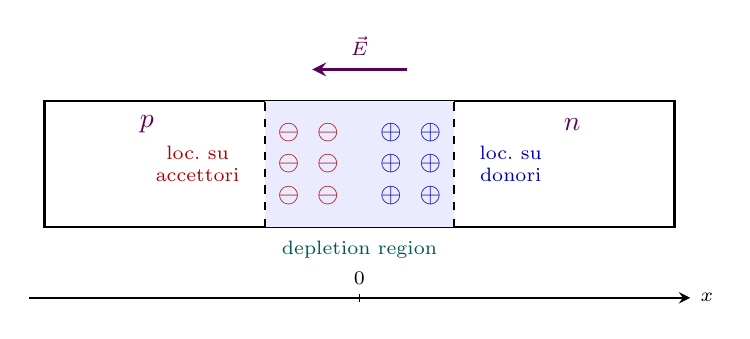
\begin{tikzpicture}[>=stealth, scale=1.0]
        % Box of the junction
        \draw[thick] (-4, -0.8) rectangle (4, 0.8);
        \draw[thick, dashed] (0, -0.8) -- (0, 0.8);
        \node[violet!70!black, font=\bfseries] at (-2.7, 0.5) {\( p \)};
        \node[violet!70!black, font=\bfseries] at (2.7, 0.5) {\( n \)};

        % Depletion region
        \fill[blue!8] (-1.2, -0.8) rectangle (1.2, 0.8);
        \draw[thick, dashed] (-1.2, -0.8) -- (-1.2, 0.8);
        \draw[thick, dashed] (1.2, -0.8) -- (1.2, 0.8);

        % Acceptor ions (negative, left of junction)
        \foreach \y in {-0.4, 0, 0.4} {
            \node[red!70!black] at (-0.9, \y) {\( \ominus \)};
            \node[red!70!black] at (-0.4, \y) {\( \ominus \)};
        }
        % Donor ions (positive, right of junction)
        \foreach \y in {-0.4, 0, 0.4} {
            \node[blue!70!black] at (0.4, \y) {\( \oplus \)};
            \node[blue!70!black] at (0.9, \y) {\( \oplus \)};
        }

        % Internal field
        \draw[->, violet!70!black, very thick] (0.6, 1.2) -- (-0.6, 1.2);
        \node[violet!70!black, anchor=south, font=\scriptsize] at (0, 1.25) {\( \vec{E} \)};

        % Labels for ion localization
        \node[red!70!black, anchor=east, font=\scriptsize, align=center] at (-1.4, 0) {loc.\ su \\ accettori};
        \node[blue!70!black, anchor=west, font=\scriptsize, align=center] at (1.4, 0) {loc.\ su \\ donori};

        % Depletion region label
        \node[teal!70!black, anchor=north, font=\scriptsize] at (0, -0.85) {depletion region};
        \node[anchor=north, font=\scriptsize] at (0, -1.25) {\( 0 \)};

        % x-axis
        \draw[->, thick] (-4.2, -1.7) -- (4.2, -1.7) node[right, font=\scriptsize] {\( x \)};
        \draw[thin] (0, -1.65) -- (0, -1.75);
    \end{tikzpicture}
    \caption{Giunzione \( p \)-\( n \): all'interfaccia si forma la depletion region, in cui restano scoperte le cariche fisse dei droganti ionizzati e si stabilisce un campo elettrico interno \( \vec{E} \) diretto dal lato \( n \) verso il lato \( p \).}
    \label{fig:giunzione_pn}
\end{figure}

Quando i due materiali vengono messi a contatto, all'interfaccia gli elettroni della regione \( n \) e le lacune della regione \( p \), in eccesso rispetto al rispettivo valore di equilibrio, diffondono attraverso la giunzione e si ricombinano. Si forma così una regione, detta \textbf{depletion region} (o \emph{regione di svuotamento}), priva di portatori liberi e in cui restano scoperte le cariche fisse degli atomi droganti ionizzati: ioni accettori negativi sul lato \( p \) e ioni donori positivi sul lato \( n \). I portatori maggioritari restano gli elettroni nella regione \( n \) e le lacune nella regione \( p \), ma sono ormai confinati al di fuori della zona svuotata.
La separazione di carica all'interno della depletion region genera un \textbf{campo elettrico interno} \( \vec{E} \) diretto dagli ioni donori positivi (lato \( n \)) verso gli ioni accettori negativi (lato \( p \)). Tale campo si oppone al moto diffusivo dei portatori e cresce finché il flusso netto attraverso la giunzione non si annulla, segnando l'equilibrio. Alla differenza di potenziale che si stabilisce attraverso la depletion region si dà il nome di \textbf{differenza di potenziale di giunzione} \( \Delta \varphi \).

Se sulla depletion region incide un fotone di energia sufficiente, esso può creare una coppia elettrone-lacuna: l'elettrone viene promosso in banda di conduzione e la lacuna resta in banda di valenza. Il campo elettrico interno separa immediatamente i due portatori, spingendo l'elettrone verso il lato \( n \) e la lacuna verso il lato \( p \), generando così una corrente fotogenerata. È questo il principio di funzionamento dei pannelli fotovoltaici.

La regione svuotata si estende per una larghezza \( W_p \) nel lato \( p \) e \( W_n \) nel lato \( n \), che in generale sono diverse. Indicando con \( N_A \) e \( N_D \) le concentrazioni di accettori e donori ionizzati, la condizione di neutralità globale del sistema impone che la carica negativa scoperta nel lato \( p \) eguagli in modulo quella positiva scoperta nel lato \( n \):
\begin{importantbox}
    \begin{equation}
        \abs{N_A \, W_p} = \abs{N_D \, W_n}
    \end{equation}
\end{importantbox}
La densità di carica spaziale \( \rho(x) \) all'interno della giunzione è quindi negativa nel lato \( p \) (carica degli accettori ionizzati) e positiva nel lato \( n \) (carica dei donori ionizzati), nulla al di fuori della depletion region.

\begin{figure}[htbp]
    \centering
    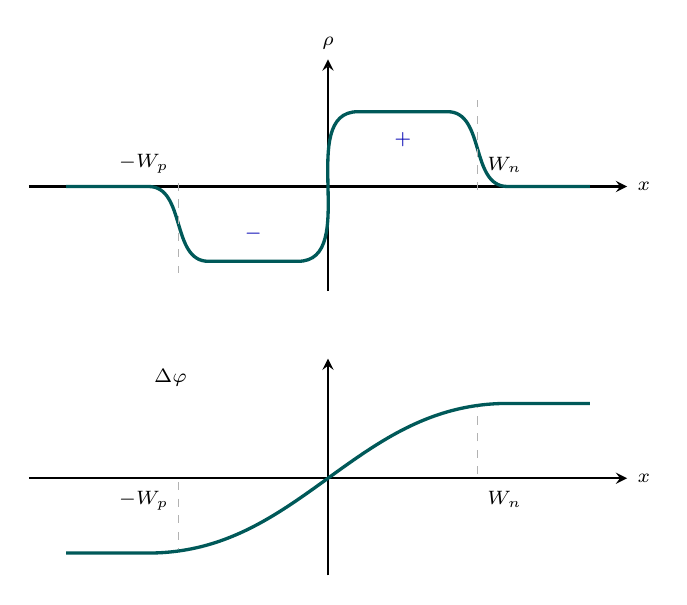
\begin{tikzpicture}[>=stealth, scale=0.95]
        % ===== Top: charge density =====
        \def\yT{2.6}
        \draw[->, thick] (-4, \yT) -- (4, \yT) node[right, font=\scriptsize] {\( x \)};
        \draw[->, thick] (0, \yT-1.4) -- (0, \yT+1.7) node[left, font=\scriptsize, anchor=south, ] {$\rho$};

        \draw[teal!70!black, very thick]
            (-3.5, \yT) -- (-2.4, \yT)
            to[out=0, in=180] (-1.6, \yT-1.0)
            -- (-0.4, \yT-1.0)
            to[out=0, in=180] (0.4, \yT+1.0)
            -- (1.6, \yT+1.0)
            to[out=0, in=180] (2.4, \yT)
            -- (3.5, \yT);

        \node[blue!70!black, anchor=south, font=\scriptsize] at (1, \yT+0.4) {\( + \)};
        \node[blue!70!black, anchor=north, font=\scriptsize] at (-1, \yT-0.4) {\( - \)};

        \draw[gray!60, dashed] (-2, \yT+0.05) -- (-2, \yT-1.15);
        \draw[gray!60, dashed] (2, \yT-0.05) -- (2, \yT+1.15);
        \node[anchor=south east, font=\scriptsize] at (-2, \yT+0.05) {\( -W_p \)};
        \node[anchor=south west, font=\scriptsize] at (2, \yT+0.05) {\( W_n \)};

        % ===== Bottom: potential =====
        \def\yB{-1.3}
        \draw[->, thick] (-4, \yB) -- (4, \yB) node[right, font=\scriptsize] {\( x \)};
        \draw[->, thick] (0, \yB-1.3) -- (0, \yB+1.6) node[left, font=\scriptsize, anchor=north, xshift = -2cm] {\( \Delta \varphi \)};

        \draw[teal!70!black, very thick]
            (-3.5, \yB-1.0) -- (-2.4, \yB-1.0)
            to[out=0, in=180] (2.4, \yB+1.0)
            -- (3.5, \yB+1.0);

        \draw[gray!60, dashed] (-2, \yB-0.05) -- (-2, \yB-0.95);
        \draw[gray!60, dashed] (2, \yB+0.05) -- (2, \yB+0.95);
        \node[anchor=north east, font=\scriptsize] at (-2, \yB-0.05) {\( -W_p \)};
        \node[anchor=north west, font=\scriptsize] at (2, \yB-0.05) {\( W_n \)};
    \end{tikzpicture}
    \caption{Densità di carica spaziale (in alto) e differenza di potenziale (in basso) lungo la giunzione \( p \)-\( n \) in funzione di \( x \).}
    \label{fig:densita_carica_pn}
\end{figure}

\subsubsection{Struttura a bande e potenziale chimico all'equilibrio}

Una volta esaurito il transiente iniziale di diffusione e ricombinazione, la giunzione raggiunge una condizione di equilibrio termodinamico. In questa condizione il \textbf{potenziale chimico} \( \mu \), che coincide con il livello di Fermi \( E_F \), assume lo stesso valore su entrambi i lati della giunzione: nello schema a bande \( \mu \) si rappresenta come una linea orizzontale costante che attraversa tutto il sistema. È proprio questa proprietà che ci permette di descrivere il materiale nel suo complesso, in assenza di campi elettrici esterni applicati.

L'allineamento di \( \mu \) impone che le bande di conduzione e di valenza, che nel cristallo \( p \) isolato sono spostate verso l'alto (poiché \( \mu \) è prossimo a \( E_v \)) e nel cristallo \( n \) verso il basso (poiché \( \mu \) è prossimo a \( E_c \)), si raccordino con una flessione continua nella depletion region. Il salto totale fra il livello di BC nel lato \( p \) e quello nel lato \( n \) corrisponde all'energia \( e V_{bi} \), dove \( V_{bi} \) è la \emph{built-in voltage} di giunzione.

\begin{figure}[htbp]
    \centering
    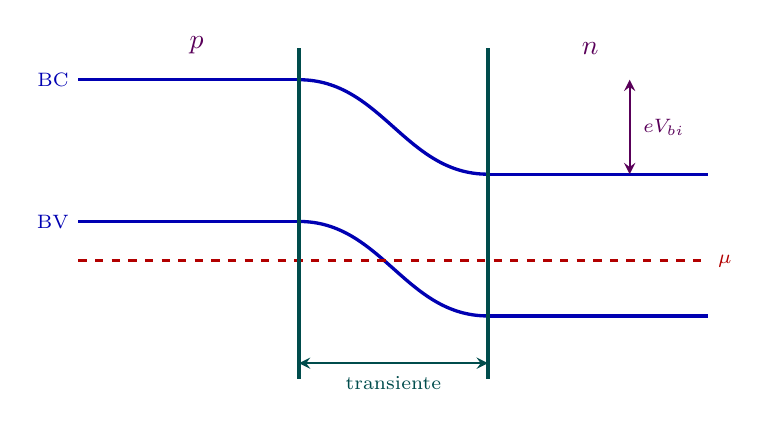
\begin{tikzpicture}[>=stealth, scale=1.0]
        % p side bands (high)
        \draw[blue!70!black, very thick] (-4, 2.0) -- (-1.2, 2.0);
        \draw[blue!70!black, very thick] (-4, 0.2) -- (-1.2, 0.2);
        % n side bands (low)
        \draw[blue!70!black, very thick] (1.2, 0.8) -- (4, 0.8);
        \draw[blue!70!black, very thick] (1.2, -1.0) -- (4, -1.0);
        % Smooth transitions through depletion region
        \draw[blue!70!black, very thick] (-1.2, 2.0) to[out=0, in=180] (1.2, 0.8);
        \draw[blue!70!black, very thick] (-1.2, 0.2) to[out=0, in=180] (1.2, -1.0);

        % Chemical potential (horizontal constant line)
        \draw[red!70!black, very thick, dashed] (-4, -0.3) -- (4, -0.3);
        \node[red!70!black, anchor=west, font=\scriptsize] at (4, -0.3) {\( \mu \)};

        % Labels
        \node[blue!70!black, anchor=east, font=\scriptsize] at (-4, 2.0) {BC};
        \node[blue!70!black, anchor=east, font=\scriptsize] at (-4, 0.2) {BV};
        \node[violet!70!black, font=\bfseries, anchor=south] at (-2.5, 2.2) {\( p \)};
        \node[violet!70!black, font=\bfseries, anchor=south] at (2.5, 2.2) {\( n \)};

        % Depletion region markers
        \draw[teal!60!black, very thick] (-1.2, -1.8) -- (-1.2, 2.4);
        \draw[teal!60!black, very thick] (1.2, -1.8) -- (1.2, 2.4);
        \draw[<->, teal!60!black, thick] (-1.2, -1.6) -- (1.2, -1.6);
        \node[teal!60!black, anchor=north, font=\scriptsize] at (0, -1.65) {transiente};

        % built-in energy gap eV_bi
        \draw[<->, violet!70!black, thick] (3.0, 2.0) -- (3.0, 0.8);
        \node[violet!70!black, anchor=west, font=\scriptsize] at (3.05, 1.4) {\( e V_{bi} \)};
    \end{tikzpicture}
    \caption{Struttura a bande della giunzione \( p \)-\( n \) all'equilibrio: il potenziale chimico \( \mu \) si allinea sui due lati e le bande si raccordano con una flessione nella depletion region. Il salto di energia \( e V_{bi} \) corrisponde alla \emph{built-in voltage} di giunzione.}
    \label{fig:bande_giunzione_pn}
\end{figure}

\subsubsection{Polarizzazione della giunzione}

Quando alla giunzione \( p \)-\( n \) si applica una differenza di potenziale esterna \( V \) si parla di \textbf{polarizzazione} (o \emph{bias}): il campo elettrico applicato si sovrappone a quello intrinseco della depletion region e ne modifica la struttura a bande in modo diverso a seconda del verso della tensione applicata.

\textbf{Polarizzazione diretta (forward bias).} Si parla di polarizzazione diretta quando il polo positivo del generatore esterno è collegato al lato \( p \) e il polo negativo al lato \( n \). Il campo elettrico applicato risulta \emph{opposto} a quello intrinseco di giunzione, riducendo l'altezza della barriera di potenziale.

\begin{figure}[htbp]
    \centering
    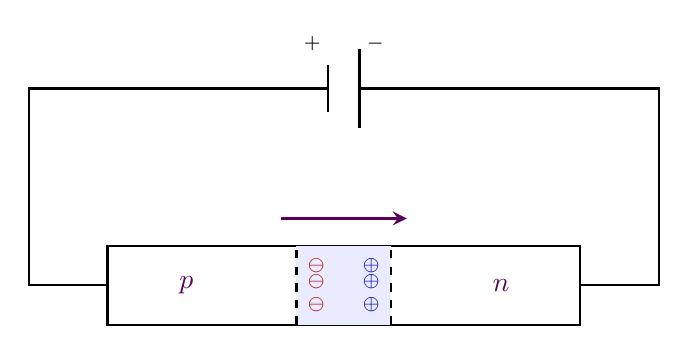
\begin{tikzpicture}[>=stealth, scale=1.0]
        % Battery (on top)
        \draw[thick] (-1.5, 2.5) -- (-0.2, 2.5);
        \draw[thick] (0.2, 2.5) -- (1.5, 2.5);
        \draw[thick] (-0.2, 2.2) -- (-0.2, 2.8);
        \draw[thick] (0.2, 2.0) -- (0.2, 3.0);
        \node[anchor=south, font=\scriptsize] at (-0.4, 2.85) {\( + \)};
        \node[anchor=south, font=\scriptsize] at (0.4, 2.85) {\( - \)};

        % Wires entering the junction from the sides
        \draw[thick] (-1.5, 2.5) -- (-4, 2.5) -- (-4, 0) -- (-3, 0);
        \draw[thick] (1.5, 2.5) -- (4, 2.5) -- (4, 0) -- (3, 0);

        % p-n junction box
        \draw[thick] (-3, -0.5) rectangle (3, 0.5);
        \draw[thick, dashed] (0, -0.5) -- (0, 0.5);
        \node[violet!70!black, font=\bfseries] at (-2, 0) {\( p \)};
        \node[violet!70!black, font=\bfseries] at (2, 0) {\( n \)};

        % Depletion region (narrower for forward bias)
        \fill[blue!8] (-0.6, -0.5) rectangle (0.6, 0.5);
        \draw[thick, dashed] (-0.6, -0.5) -- (-0.6, 0.5);
        \draw[thick, dashed] (0.6, -0.5) -- (0.6, 0.5);

        \foreach \y in {-0.25, 0.05, 0.25} {
            \node[red!70!black, font=\scriptsize] at (-0.35, \y) {\( \ominus \)};
            \node[blue!70!black, font=\scriptsize] at (0.35, \y) {\( \oplus \)};
        }

        % External field arrow inside the device (from + terminal to - terminal: p to n)
        \draw[->, violet!70!black, very thick] (-0.8, 0.85) -- (0.8, 0.85);
    \end{tikzpicture}
    \caption{Polarizzazione diretta (forward bias): il polo positivo è collegato al lato \( p \) e il polo negativo al lato \( n \). La regione di svuotamento si riduce in ampiezza.}
    \label{fig:forward_bias}
\end{figure}

Il nome ``polarizzazione diretta'' deriva dal fatto che la tensione applicata ha lo stesso verso della tendenza naturale di moto dei portatori maggioritari nei rispettivi lati: gli elettroni del lato \( n \) sono spinti verso la giunzione e le lacune del lato \( p \) sono spinte nella stessa direzione, contrastando il campo interno e \emph{restringendo} la depletion region.

\textbf{Polarizzazione inversa (reverse bias).} Si parla di polarizzazione inversa quando il polo positivo del generatore è collegato al lato \( n \) e il polo negativo al lato \( p \). Il campo applicato risulta in questo caso \emph{concorde} a quello intrinseco di giunzione, rafforzandolo.

\begin{figure}[htbp]
    \centering
    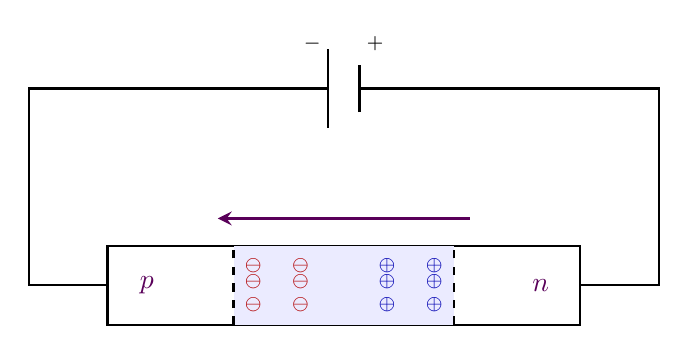
\begin{tikzpicture}[>=stealth, scale=1.0]
        % Battery (on top)
        \draw[thick] (-1.5, 2.5) -- (-0.2, 2.5);
        \draw[thick] (0.2, 2.5) -- (1.5, 2.5);
        \draw[thick] (-0.2, 2.0) -- (-0.2, 3.0);
        \draw[thick] (0.2, 2.2) -- (0.2, 2.8);
        \node[anchor=south, font=\scriptsize] at (-0.4, 2.85) {\( - \)};
        \node[anchor=south, font=\scriptsize] at (0.4, 2.85) {\( + \)};

        % Wires entering the junction from the sides
        \draw[thick] (-1.5, 2.5) -- (-4, 2.5) -- (-4, 0) -- (-3, 0);
        \draw[thick] (1.5, 2.5) -- (4, 2.5) -- (4, 0) -- (3, 0);

        % p-n junction box
        \draw[thick] (-3, -0.5) rectangle (3, 0.5);
        \draw[thick, dashed] (0, -0.5) -- (0, 0.5);
        \node[violet!70!black, font=\bfseries] at (-2.5, 0) {\( p \)};
        \node[violet!70!black, font=\bfseries] at (2.5, 0) {\( n \)};

        % Depletion region (wider for reverse bias)
        \fill[blue!8] (-1.4, -0.5) rectangle (1.4, 0.5);
        \draw[thick, dashed] (-1.4, -0.5) -- (-1.4, 0.5);
        \draw[thick, dashed] (1.4, -0.5) -- (1.4, 0.5);

        \foreach \y in {-0.25, 0.05, 0.25} {
            \node[red!70!black, font=\scriptsize] at (-1.15, \y) {\( \ominus \)};
            \node[red!70!black, font=\scriptsize] at (-0.55, \y) {\( \ominus \)};
            \node[blue!70!black, font=\scriptsize] at (0.55, \y) {\( \oplus \)};
            \node[blue!70!black, font=\scriptsize] at (1.15, \y) {\( \oplus \)};
        }

        % External field arrow (from + to -: n to p)
        \draw[<-, violet!70!black, very thick] (-1.6, 0.85) -- (1.6, 0.85);
    \end{tikzpicture}
    \caption{Polarizzazione inversa (reverse bias): il polo positivo è collegato al lato \( n \) e il polo negativo al lato \( p \). La regione di svuotamento si allarga.}
    \label{fig:reverse_bias}
\end{figure}

In polarizzazione inversa la depletion region si \emph{allarga}: il campo esterno spinge gli elettroni del lato \( n \) lontano dalla giunzione e le lacune del lato \( p \) lontano dall'interfaccia, lasciando scoperte un maggior numero di cariche fisse di drogante.

L'allargamento della regione di svuotamento è particolarmente utile nelle applicazioni fotovoltaiche: la depletion region è infatti il volume attivo in cui i fotoni incidenti possono creare coppie elettrone-lacuna che il campo intrinseco separa, generando corrente. Più ampia è la depletion region, più fotoni vengono assorbiti utilmente e più efficiente risulta la conversione fotovoltaica. Per questo motivo le celle solari sono in genere progettate per operare in regime di polarizzazione inversa (o nulla, a circuito aperto), in modo da massimizzare il volume di raccolta.

